\documentclass{ucbthesis}
\usepackage{biblatex}

% Double spacing, if you want it.
% \def\dsp{\def\baselinestretch{2.0}\large\normalsize}
% \dsp

% If the Grad. Division insists that the first paragraph of a section
% be indented (like the others), then include this line:
% \usepackage{indentfirst}

\newtheorem{theorem}{Jibberish}

\bibliography{references}

\hyphenation{mar-gin-al-ia}

\begin{document}

% Declarations for Front Matter

\title{An Internet-Spanning Content Distribution Mechanism for IoT}
\author{Griffin Potrock}
\degreesemester{Spring}
\degreeyear{2018}
\degree{Master of Science}
\chair{Professor John Kubiatowicz}
\othermembers{Professor John Wawrzynek}
\numberofmembers{2}
\prevdegrees{B.S. (University of California, Berkeley) 2017}
\field{Electrical Engineering and Computer Science}
\campus{Berkeley}

% For a masters thesis, uncomment (remove the % at the beginning of)
% the following line.  This affects the title and approval pages,
% which by default calls this a "dissertation", not a "thesis".

%\itsamasters

% The title page generated by LaTeX is now acceptable for handing in.
% (This was not always the case).

\maketitle
\approvalpage
\copyrightpage

% (This is included by thesis.tex; you do not latex it by itself.)

\begin{abstract}

% The text of the abstract goes here.  If you need to use a \section
% command you will need to use \section*, \subsection*, etc. so that
% you don't get any numbering.  You probably won't be using any of
% these commands in the abstract anyway.

Low-cost, Internet-connected devices are rapidly proliferating in a computing mega-trend known as the Internet of Things (IoT). While the IoT offers great opportunities, from smart cities to smart homes, it also offers many new computing challenges.  These challenges include handling larger numbers of devices; handling more upstream and inter-device communication; and managing the secure storage and distribution of rapidly increasing amounts of data. 

The Global Data Plane (GDP) project seeks to re-architect the networking infrastructure of the Internet to accommodate these trends. The GDP relies on replicated, append-only logs. In addition to being a durable data store, these logs are often used as a single-writer publish/subscribe mechanism. 

This thesis proposes new mechanisms for adapting publish/subscribe to the networking challenges of IoT. We detail design choices for a new overlay-based multicast system, the Secure Content Distribution Tree (SCDT), that are both novel and thoroughly grounded in existing literature and experience to ensure viability. We also propose new, scalable mechanisms for providing reliability in such a system.  While our evaluation focuses on demonstrating the viability of our multicast architecture and reliability mechanisms through simulations, we also include discussions on security and deployment.

\end{abstract}


\begin{frontmatter}


\tableofcontents
\clearpage
\listoffigures
\clearpage
\listoftables

\begin{acknowledgements}
Thanks Kubi, Nitesh, Eric, Rick, and Ken.
\end{acknowledgements}

\end{frontmatter}

\pagestyle{headings}

% (Optional) \part{First Part}

\chapter{Introduction}

\section{Background}

The Internet of Things is a computing macrotrend poised to change the way we interact with computing environments and reshape the Internet. While the push toward cloud computing has lead to increasing centralization of the Internet into a handful of data centers, the proliferation of IoT devices is pushing computation and data flows back toward the network edge.

IoT applications may be worth up to \$11 trillion by 2025. However, 40\% of this value relies on coordination between IoT systems \cite{McKinsey}. Developers face any a number of challenges in capturing this value. An effective IoT deployment cannot simply be a direct connection between every individual IoT device and a cloud data center \cite{kubi}. Round trips to the cloud are inefficient in  latency, bandwidth, and network stress, limiting scalability and imposing deployment constraints. IoT devices are often embedded, low-power devices with low duty-cycles, making ensuring reliability and durability of data at best an unnecessary energy drain and at worst a debilitating constraint. Furthermore, routing to and utilizing the cloud comes with a number of privacy and security risks.

\subsection{Latency, Bandwidth, and Scalability}
In many cases, IoT devices can only realize their potential when they are able to distribute their data to thousands or millions of subscribers efficiently. For example, a temperature sensor might need to publish current temperature readings to every HVAC system in a neighborhood, or an air quality sensor might need to send pollution warnings to citizens in a wide area. 

Many IoT applications involve real-time latency constraints, which almost entirely preclude going to the cloud to access data.  A traditional option is for the device originating the record to store and retransmit it to interested nearby devices that fail to receive the original transmission.  This is a poor option given the constraints of such end-devices.  If neither the cloud nor the original device are a reasonable source of caching and retransmission, that means that responsibility must be pushed elsewhere in the network.

Since many IoT applications involve nearby devices intercommunicating, round trips to the cloud make little sense. Such a solution would place undo stress on the border gateways of the network, requiring beefy links to the Internet. This is an unnecessary expense and a serious problem for remote deployments.

\subsection{Device Constraints}
The uniformity of the phrase ``Internet of Things" obscures the massive variety of devices and software that will be deployed in the IoT, not only across manufacturers and developers but also between different versions deployed at different times.  Achieving consistent performance is difficult in the presence of such heterogeneity. Some popular controllers such as Raspberry Pi \cite{RaspberryPi} and BeagleBone \cite{BeagleBone} are powerful enough to run full desktop Linux distributions.  Others, such as Telos B \cite{Telos}, which remains popular in the wireless sensor network research community, focus on minimizing power consumption.  Even low-power motes have a variety of choices when it comes to operating systems, including TinyOS \cite{tinyos}, Contiki \cite{contiki}, and RIOT \cite{riot}.  Further, such motes may only be able to transmit occasionally due to power constraints, such as motes that use power harvesting techniques.

Developers currently looking to build heterogeneous IoT systems must develop solutions that can coordinate across an ever increasing mix of hardware and software deployed in the field.  The low duty cycle of some IoT devices can make direct inter-device communication difficult.

In many cases, IoT devices will also have to ensure the reliability and durability of their data. Having all data subscribers communicate directly with the publisher, such as with TCP, is essentially impossible due to inconsistent timing and a lack of sufficient processing power and bandwidth on virtually all IoT devices to service heavy traffic. 

\subsection{Privacy and Security}
Security requirements can impose significant constraints on any networking protocol for the IoT.  Many applications will require data confidentiality, necessitating that all data be encrypted.  This encryption scheme must be scalable to communication with thousands of devices.

Encryption alone, however, does not preclude side-channel attacks or traffic analysis attacks \cite{sidechannel}.  One example might be a device that writes an encrypted ``open/close" command to a door, allowing anyone who can snoop on the encrypted traffic to determine when someone enters/exits the building without decrypting the data.  Corporations in particular frequently do not want to entrust their proprietary data to external storage or allow it to be routed outside their corporate network, even when it is encrypted.  Data regulations in some countries restrict what data can flow across international borders \cite{itif}. Even within countries, any IoT data security scheme must allow some restriction on where data is allowed to flow, or set up secure, noise-injected channels between trusted nodes.

\section{Related Work}

Our solutions build upon the large body of academic literature and industry experience in multicast. Multicast is fundamentally a simple concept: rather than sending packets to individual destinations, the network uses intermediate routers as fanout points to reduce the strain on any one router. Unfortunately, this concept has seen limited adoption due to a number of implementation and deployment issues. There are two fundamentally different categories of multicast schemes: IP multicast and overlay multicast. Either can be used in a publish/subscribe system.

\begin{table}
	\begin{center}
		\begin{tabular}{|c|c|c|}
			\hline
			 & \textbf{IP Multicast} & \textbf{Overlay Multicast} \\
			\hline
			\textbf{Incrementally Deployable} & No & Yes \\
			\hline
			\textbf{Easily Support Firewalls/NATs} & No & Yes \\
			\hline
			\textbf{Network Stress} & Lower & Higher \\
			\hline
			\textbf{Average Stretch} & Lower & Higher \\
			\hline
		\end{tabular}
	\end{center}
	\caption{Comparison of IP multicast and overlay multicast.}
\end{table}


\subsection{IP Multicast}
\label{ip-multicast}
IP multicast is a network-level multicast concept that has been a popular research topic since at least the 1990s. Despite the uniformity implied by the name, there is no one single IP multicast protocol or technology. Rather, IP multicast instead refers to a collection of protocols. In general terms, these protocols rely on constructing forwarding tables at individual routers that map an IP multicast address to a series of next-hop routers. IP multicast addresses are specified in RFC 1112 \cite{RFC1112}; specifically addresses ranging from 224.0.0.0 to 239.255.255.255 are pointed to zero or more end-hosts.

Perhaps the most common IP multicast deployment involves Protocol Independent Multicast (usually Sparse Mode) \cite{RFC2362} and Internet Group Management Protocol (IGMP) \cite{RFC4605}. Although they operate at the network level, these protocols operate above the protocols that actually construct IP forwarding tables. Therefore, they can be used in conjunction with most routing protocols, such as OSPF \cite{RFC2328}, IS-IS \cite{ISO10589}, and RIP \cite{RFC2453} - hence the ``Protocol Independent" portion of the name. 

In brief, PIM-SM works by having routers with downstream clients send Join/Prune requests towards a designated Rendezvous Point (RP) and using these requests to build the forwarding tables. Data is then multicasted by having each router forward the data on all interfaces that have downstream clients in the multicast group.

There are any number of alternative and supplementary protocols in the IP multicast space. PIM Dense Mode (PIM-DM) \cite{RFC3973}, Border Gateway Multicast Protocol (BGMP) \cite{RFC3913}, Multicast Open Shortest Path First (MOSPF) \cite{RFC1584}, Distance Vector Multicast Routing Protocol (DVMRP) \cite{RFC1075}, Core Based Trees (CBT) \cite{RFC2201}, and Ordered Core Based Trees (OCBT) \cite{OCBT} all fill similar niches with varying degrees of success.  PIM can also be supplemented with protocols like Multicast Source Discovery Protocol (MSDP) \cite{RFC4611}, which interconnects PIM-SM domains. Multicast Listener Discovery Protocol (MLDP) \cite{RFC4604} is essentially the IPv6 version of IGMP.

A number of reliability schemes have been implemented on top of IP multicast, and are overwhelmingly based on negative acknowledgments (NAKs). NACK-Oriented Reliable Multicast (NORM) \cite{RFC5740} handles reliability by asking receivers to send a negative acknowledgment to request retransmission when a missed packet is detected. Pragmatic General Multicast (PGM) \cite{RFC3208} also uses nacks but trades off reliability guarantees for performance. Scalable Reliable Multicast (SRM) \cite{SRM} includes stronger locality principles: receivers recover by multicasting a repair request, and the missing data is retransmitted by any host that has received the packet.  Excessive repair requests/retransmissions are suppressed using exponential backoffs.

None of these protocols have seen much deployment outside of individual organization networks, let alone an Internet-spanning deployment that would be needed in an IoT world. The biggest problem has always been the deployment of multicast-capable routers. Since IP multicast is network-level, generally all or at least most routers in the network must be able to ``speak" the required protocols. Similar to IPv6, which despite substantial effort reached just 10\% deployment by its 20th anniversary \cite{ArsTechnica}, IP multicast cannot be fully effective until a large portion of the Internet adopts it, but few ISPs want to invest in a protocol with vague future returns. This is the primary reason IP multicast has seen some limited deployments, such as in corporate networks where the deployment can be controlled by a single entity, but has not been widely deployed in the broader Internet. Other limiting factors on IP multicast include but are not limited to difficulties handling interdomain routing (and who will pay for it); problems handling NATs and firewalls; and security/authorization challenges \cite{MulticastProbs}.

\subsection{Overlay Multicast}
Overlay multicast (also called Application Level Multicast or Application Layer Multicast) schemes arose to mitigate some of the problems faced by IP multicast schemes. Overlay multicast utilizes the same fundamental concept as IP multicast, using intermediate routers as fanout points to improve network efficiency. As the name suggests, overlay multicast schemes operate on overlay networks \cite{overlay}; they are application-level, rather than network-level, protocols. 

The biggest advantage of this approach is that it eliminates the deployment problems faced by IP multicast; ``multicasts" actually take the form of a series of unicast transmissions to specific destination routers, routed over IP, which then further propagate the transmission. Therefore, a handful of hosts running overlay multicast software can be deployed and reap (some of) the benefits of multicast without having to deploy IP multicast-enabled hardware throughout the network.

One of the biggest challenges with overlay multicast is that the notion of neighboring nodes is not as intuitive as it is in IP multicast. For instance, simply routing a join request towards a rendezvous point (as PIM-SM does) does not guarantee that the packet will ever encounter a router running the overlay multicast software before reading the RP, reducing such a scheme to little better than unicast. In addition, overlay multicast is inherently less efficient than IP multicast because overlay multicast does not fully consider the underlying network the way IP multicast can.

There have been a number of influential overlay multicast implementations. Scribe \cite{scribe} builds a multicast tree on top of Pastry \cite{pastry}, a Distributed Hash Table (DHT) implementation with locality properties. By routing along Pastry towards a rendezvous point, Scribe constructs a multicast tree from the union of the routes along the DHT. Overcast \cite{overcast} takes a different approach. Joining nodes will contact the root of the overcast tree and sample the connection bandwidth. The joining node then begins a series of rounds in which it will sample the current parent node's children and attach itself to the closest child that does not significantly reduce bandwidth. Narada \cite{narada} generates a connected graph among the nodes called a mesh and constructs spanning trees from there.

\subsection{Publish/Subscribe Systems}
\begin{table}
	\begin{center}
		\begin{tabular}{|c|c|c|c|c|}
			\hline
			& \textbf{GDP} & \textbf{RabbitMQ} & \textbf{Kafka} & \textbf{ZeroMQ} \\
			\hline
			\textbf{Data Distribution} & Push & Push & Pull & Pull \\
			\hline
			\textbf{Data Structure} & Append-Only Log & Queue & Append-Only Log & Queue \\
			\hline
			\textbf{Data Filtering} & No & Yes & Yes & No\\
			\hline
			\textbf{Edge-Ready} & Yes & No & No & No \\
			\hline
		\end{tabular}
	\end{center}
	\caption{Comparison of publish/subscribe systems.}
\end{table}

The pub/sub architecture \cite{pubsub} is a frequently used communications model for distributed applications. As the name suggests, subscribers register interest in specific events, and are notified of relevant events created by publishers. While the model is simple, there are many different implementations that favor different design constraints. Dedicated pub/sub systems include RabbitMQ, Apache Kafka, and ZeroMQ.

RabbitMQ \cite{amqp, amqp-disc} and Kafka \cite{kafka} are both pub/sub infrastructures. There are several similarities, including having a similar architecture based on queues and message brokers. The biggest fundamental difference between the two is that RabbitMQ brokers push data to subscribers; in Kafka, clients must request data from the brokers. Both are primarily centrally deployed (e.g. in data centers) and are mainly scaled by increasing the number of brokers.

ZeroMQ \cite{zeromq} takes a fairly different approach. When configured to use multicast, subscribers attach to the multicast tree via multicast switches; publishers send data to these multicast switches to forward through the network. These switches use Pragmatic General Multicast (PGM) \cite{RFC3208}, discussed briefly in~\autoref{ip-multicast}, to distribute data. Unfortunately, ZeroMQ inherits many of the issues associated with PGM. ZeroMQ cannot generally be deployed on top of an existing network because of its reliability on IP multicast. Publishers have no way to determine when subscribers join, fail, or reconnect. Subscribers have no ability to communicate with publishers to control the rate of messages; they must either receive published data at full speed or drop packets.

\section{Motivation}
\label{motivation}
This thesis argues for a new approach to multicast, primarily in order to enable a more efficient publish/subscribe mechanism for IoT. Decades of work on IP multicast, however, have produced lackluster results in real-world deployments, with the biggest roadblock being the inability to incrementally deploy a multicast service. Overlay multicast schemes were created to solve these problems.

However, existing overlay multicast schemes remain limited in their use cases. None target the level of scale necessary for the Internet of Things. When it was introduced, Overcast \cite{overcast}, for instance, was not evaluated on real deployments of significant size, and only simulated on up to 600 nodes. Multicast groups in the IoT could grow to thousands or even millions of nodes. Even without considering such large groups, with the number of Internet-connected IoT devices surpassing 31 billion \cite{ihs} in 2018, smaller multicast groups will often be sharing the same infrastructure, so multicast mechanisms must still be relatively lightweight and efficient.

Further, existing overlay multicast mechanisms are targeted at a non-mobile publisher maximizing throughput to subscribers. Taking full advantage of the Internet of Things will require pushing computation and networking to the edge. In many cases, this will mean an IoT multicast scheme must rapidly adapt to a mobile publisher. Perhaps even more significantly, developers will need the ability to rapidly push data to local devices. IoT devices in the same vicinity may need to interact with each other in real time, such as a smart home that turns on a light when a user opens the door or streams security camera footage to the living room TV. 

Devices further away are less likely to have real-time dependency on the data. This leads us to propose a shift: that an IoT multicast scheme should prioritize delivering data to local subscribers over subscribers further away. We further argue that, given the relatively small or infrequent messages published by many IoT devices (e.g. a temperature sensor publishing readings once per minute), an IoT multicast should prioritize latency over bandwidth. Of course, latency is determined not just by the route packets take but also by the stress on the network, the fanout at any individual node, and the quality of links (if the scheme is reliable, lossy links will require more retries). We argue that the metric to optimize is \textit{stretch}. Stretch is defined as:

\[\frac{Optimal\: Route\: Latency}{Actual\: Route\: Latency}\]

We measure stretch for a given node in practice using:

\[\frac{(Node\: Latency\: to\: Parent) + (Parent\: Latency\: to\: Publisher)}{Node\: Latency\: to\: Publisher}\]

By setting a worst case stretch value, a multicast scheme can force traffic to route through non-optimal routes in order to improve fanout and reduce stress, while simultaneously preventing long, snaking multicast trees that reduce latency.

Finally, existing multicast implementations have not paid sufficient attention to security concerns. Multicast schemes face some of the same security concerns as other applications, specifically ensuring confidentiality and authenticity of data transmitted over the network. However, the solutions that work in unicast do not apply directly to multicast. The publisher cannot negotiate a separate key for every subscriber in a system with any amount of scale.  Using a shared symmetric key for the group raises the question of how to distribute such a key to new subscribers and revoke access from other subscribers. 

Encryption alone cannot prevent side-channel or traffic analysis attacks. With many organizations loathe to give up access to their data (and some prevented from doing so by law), networking schemes to restrict the flow of data have a clear use case. Existing multicast solutions (and many networking solutions in general) do not take trust of the underlying network into account in routing. While assuming the underlying network to be untrustworthy has been the traditional network security assumption, relying on end-to-end encryption solutions alone is increasingly becoming untenable.

Our design of a new, edge-focused multicast is developed in conjunction with and targeted for the Global Data Plane (GDP) project, a publish/subscribe architecture for the Internet of Things (see~\autoref{gdp}). The GDP seeks to shift the publish/subscribe model to favor the edge over data centers; as such, a new multicast system fitting this model was necessary.



\chapter{The Global Data Plane}

\section{GDP Architecture for the Internet of Things}



\section{Multicast in the GDP}



\chapter{Secure Content Distribution Trees}

\section{Architecture}
In this section, we outline the design of SCDTs.  We make no claim that these solutions are optimal; rather, we chose these design patterns with implementation, deployment, and scalability in real-world environments in mind.

The fundamental SCDT structure is a multicast tree constructed out of an incrementally deployable overlay network \cite{overlay} of routers and end-devices running SCDT software.  The goal of this tree is to support a publish/subscribe model with a single, mobile publisher and a large number of subscribers.  We argue for scalable tree-building mechanisms that can support reliable subscribers without bottlenecking the network.  Our reliability design is based on well-researched negative acknowledgment schemes, with some changes to improve scalability for large numbers of IoT devices.  Finally, we pay particular attention to securing SCDTs.

\begin{figure}[t]
	\begin{center}
		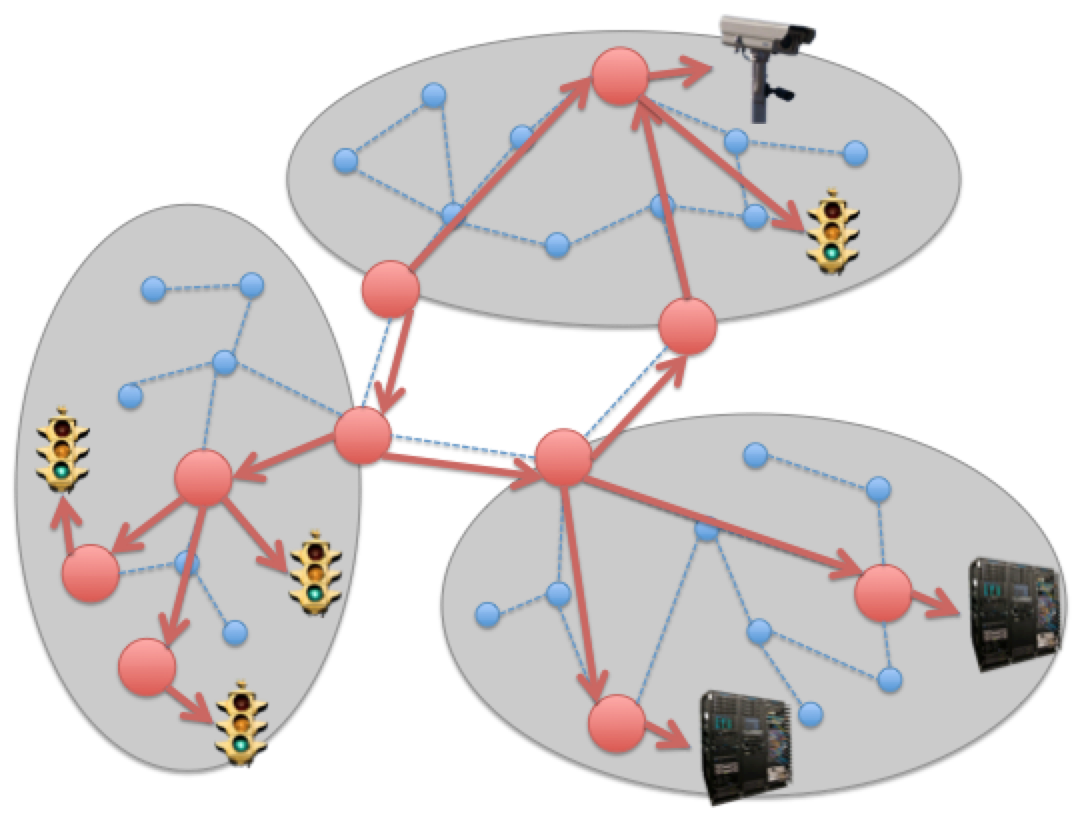
\includegraphics[scale=0.5]{network_example_2}
	\end{center}
	\vspace{-1.2em}
	\caption{\small \itshape An example SCDT running over a physical network with a traffic camera publishing data.  The overlay network  considers only the arrow links, which represent parent-child links.  Legend: large nodes are running SCDT software; small nodes are not running SCDT software; arrow lines are overlay links;  dashed lines are physical links; ovals are trusted domains.}
	\vspace{-1.5em}
	\label{fig:architecture}
\end{figure}

\subsection{Heuristic, Adaptable Multicast}
\label{adaptable-multicast}

SCDTs rely on constructing overlay multicast trees to distribute data to
large numbers of end-devices.  We show an example in~\autoref{fig:architecture}, a 
``smart city" \cite{smart-city}
deployment where street cameras must coordinate with traffic lights at the same
intersection, traffic lights of neighboring intersections, and central servers
far away.  While~\autoref{fig:architecture} only draws a half-dozen end devices, 
the analogy holds
for thousands of end-devices across a smart city, including all traffic lights,
crosswalks, and public transit systems.  Building multicast trees on top of
overlay networks has received significant study in the past \cite{overcast,
	scribe, RFC3208}.  However, these protocols often have questionable scalability, require significant work at the root of the tree, require IP multicast to be running underneath, or disregard latency or security concerns.

Building optimal multicast trees would require unrealistic amounts of overhead
at the scale we are considering.  Instead, SCDTs use heuristic methods.  We describe the characteristics necessary for an IoT
multicast tree building protocol with some similarity to that in
\cite{overcast}, but with several critical modifications.  Subscribers (and
routers serving subscribers) attach to a nearby node in the SCDT and
migrate up or down the tree to best satisfy its latency and bandwidth
constraints.

Unlike many other solutions, we argue for a multicast model in which the
publisher can move in the network and reattach to the SCDT in a different
location.  There are three key benefits to this model.  First, it allows
publishers to be  without having to regularly rebuild the entire tree.
Second, it allows nearby nodes (e.g. those with real-time constraints) to
receive data quickly, while still allowing more distant nodes to eventually
receive data.  Third, in the event of a break somewhere up the tree, nearby
devices can still receive data quickly while the tree adapts.  For instance, 
in~\autoref{fig:architecture} a network fault which isolates the local 
intersection from the rest of
the network should not cause interrupt service at the local intersection; instead, while
it may reduce the effectiveness of nearby intersections which are no longer
receiving the data, the local system can continue to function.

We also argue for a publisher/subscriber model in which there is only one
publisher and arbitrarily many subscribers. This greatly simplifies tree
construction and makes it easier to implement a mobile publisher.

End-devices themselves are not the true leaves of the SCDT.  Rather, the routers
these devices connect to should be considered the leaves of the SCDT.  Since
routers are often plugged-in and wired-in, this change in structure allows SCDTs
to impose some processing load on the leaves without compromising low-power or
low-resource devices.  The leaves can determine for themselves when and how
their heterogeneous end-devices should receive data.

Latency should not be disregarded.  Network operators should be able to tune
their devices for a worst case latency before
optimizing for bandwidth.  Latency may even be a more important factor than
bandwidth when considering IoT devices which send data to subscribers relatively
infrequently.  Rather than trying to sample bandwidth, nodes should simply
attach to a nearby parent.  If they are unable to satisfy latency constraints or
keep up with the data stream at their current location, they should migrate
up/down the tree as necessary.  Such a strategy avoids prematurely optimizing
for bandwidth in trees which are only occasionally sending data, and helps to
avoid unnecessarily long, snaking trees.  In~\autoref{fig:architecture}, SCDTs 
provide low latency
to the nearby traffic light which requires current data; meanwhile, devices
further away with looser latency constraints will accrue greater bandwidth
advantages. 

Rather than considering the Internet as a more or less randomly
distributed graph of nodes, SCDTs consider the network as a series of
interconnected, hierarchical domains of ownership.  Domains are analogous to
Autonomous Systems \cite{RFC1930} and in many cases network operators might
determine domain and AS boundaries to be the same.  Border gateways of
domains/ASes provide a natural choice for multicast points, and can help to
service join requests and maintenance, reducing strain at higher levels of the
SCDT.  While this might provide a single point of failure (or relatively few
points of failure), if the border gateways of an AS fail then there is no access to the
broader Internet anyway.  See~\autoref{domains} for a discussion of the security aspects of domains.

\begin{figure}[t]
	\begin{center}
		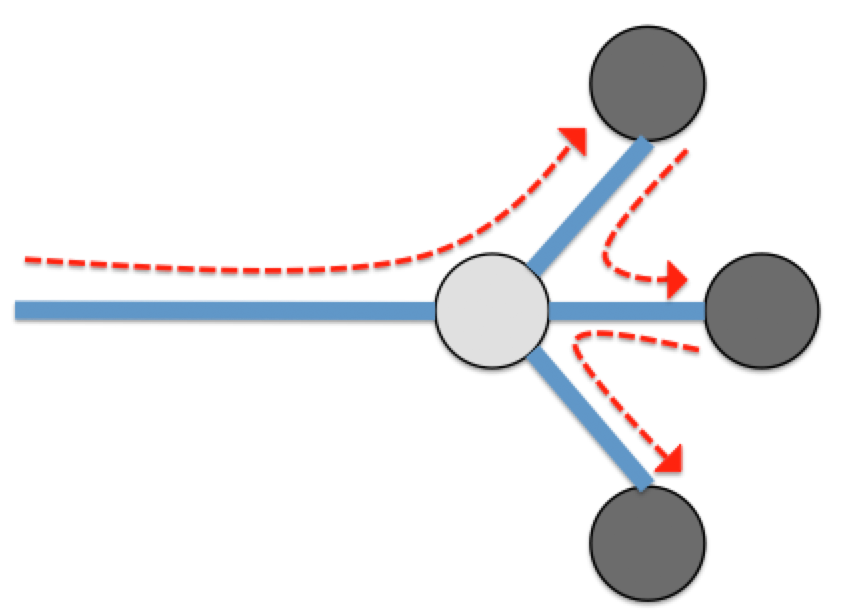
\includegraphics[scale=0.5]{poor_routing.png}
		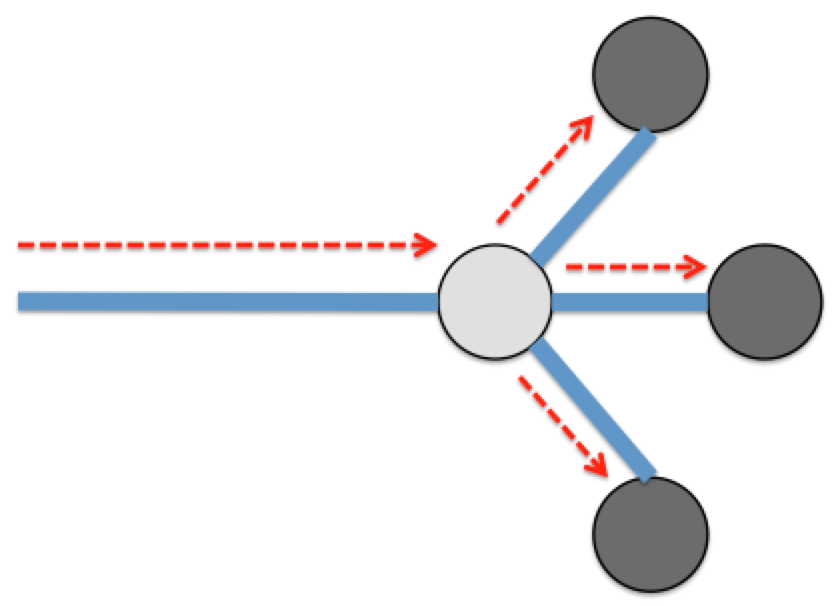
\includegraphics[scale=0.5]{good_routing.png}
	\end{center}
	\vspace{-1.3em}
	\caption{\small \itshape Left: Overlay routing without forced participation, requiring unnecessary retransmission.  Right: Overlay routing with forced participation.  Children receive the packet faster, and the non-subscribing router handles fewer packets.  Legend: light gray routers are not subscribing; dark gray routers are subscribing; solid lines are physical links; dashed lines show packet flow.}
	\vspace{-1em}
	\label{fig:overlay-tree}
\end{figure}

We argue that overlay network routers that are not themselves subscribers to the
data on a particular SCDT should be eligible to be drafted into service to
increase tree efficiency. ~\autoref{fig:overlay-tree} demonstrates a simple 
scenario in which
router promotion would improve routing efficiency.  By analyzing the way overlay
links are constructed over the physical network, the SCDT can identify router
promotions which would increase efficiency.  The ability to promote unknown
routers relies on the construction of trusted domains; only routers within the
trusted domain should be eligible for promotion.

\subsection{Secure Resolution Systems}
\label{sec-resolution-system}

A key construct of the SCDT system is the Secure Resolution System (SRS)
provided by each domain.  SRSes are roughly analogous to DNS, in that they are a
hierarchical address resolution scheme.  A new subscriber can contact its local
SRS for information on border routers and attachments points for the desired
SCDT.  If the subscriber is the first in its domain, the SRS will point it to
another SRS higher up the hierarchy.

Having all subscribers join the tree by contacting the root is cumbersome and slow. However, because SCDTs involve migrating between attachment points, new subscribers could theoretically use any existing node to join the tree. The closer the initially contacted node is to the ultimate attachment point, the more quickly the SCDT will converge to an optimal placement. The SRSes provide a simple way to find good attach points while allowing local administrators to configure the joining process if necessary. For instance, the local administrator might designate a single node as the domain attach point under the assumption that the domain will always keep that node running; or the administrator could configure a dynamic response based on the knowledge the SRS has about currently active nodes in the domain.

The implementation of the SRS is up to the domain administrator.  A basic version on an SRS could simply be a database on a single server that contains border router information and pointers to other SRSes up the
hierarchy; the IP address of this server could then be hard coded into all
devices in the domain.  A better version could be built using a Distributed Hash
Table \cite{chord, tapestry}.

\subsection{Durability and Replication}
\label{durability-replication}

While many IoT applications involve sending data for immediate consumption, it is also necessary to maintain a store of records somewhere in the network.  The reasons for supporting such replicated, durable storage are threefold.  First, end-devices which require reliable service need a final ground-truth to consult when data has already been completely purged from network caches.  This is also the case for end-devices which go down and come back up later and need to consult data long forgotten by the routing infrastructure or even the publisher itself.  Second, many users will be interested in using analytics to derive insights from historical data.  Third, some devices may only need certain pieces of data, and do not want to be fully joined to the SCDT.

Ideally, the SCDT can perform double duty, transporting data to interested end-devices as well as these ground-truth durable replicas.

\subsection{Mobile Writer}
\label{mobile-writer}
\begin{figure}[t]
	\begin{center}
		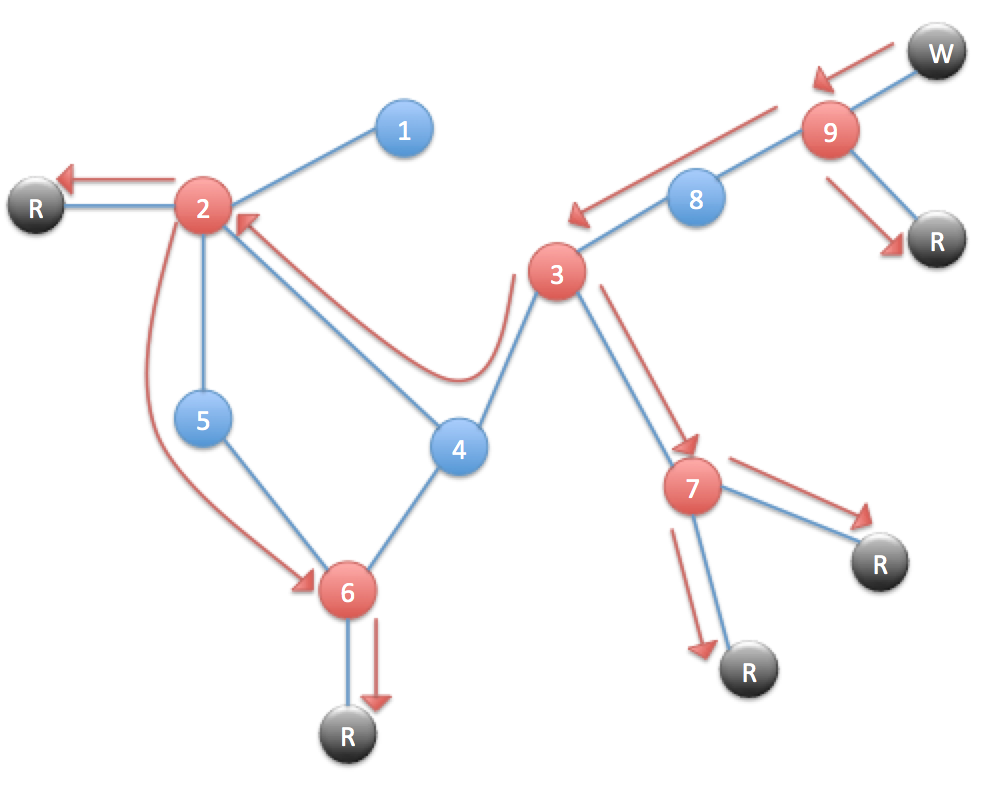
\includegraphics[scale=0.5]{physical_network.png}
		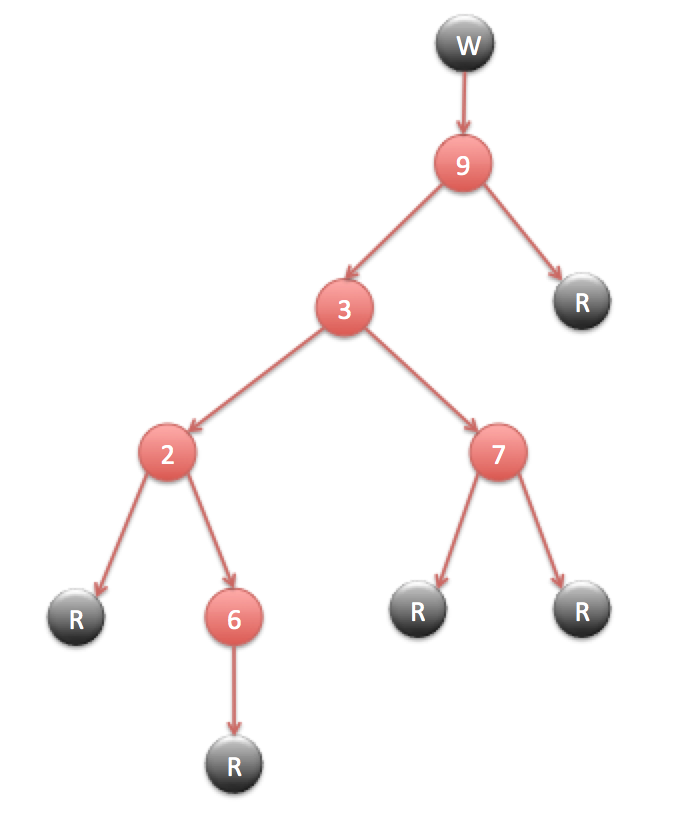
\includegraphics[scale=0.5]{overlay.png}
	\end{center}
	\vspace{-1.3em}
	\caption{\small \itshape Left: A physical network with SCDT nodes running on some machines.  Right: The logical tree formed from that network.  Legend: blue routers are not subscribing; red routers are subscribing; solid lines are physical links; dashed lines show packet flow.}
	\vspace{-1em}
	\label{fig:multicast-tree}
\end{figure}
We have designed SCDTs with a mobile publisher in mind. This means that a self-driving car or robot can reattach to the network elsewhere in the tree quickly. When the publisher rejoins the tree, routers can easily convert their previous parent connection to a child connection (since they're now receiving data from somewhere else). As the receivers continuously test their connections and migrate to better positions, the tree will eventually reform to a shape that better reflects the publisher's new position.

\section{Security Implications}
\subsection{Denial of Service}
\label{denial-of-service}
Denial of service and amplification attacks are a major risk in SCDTs, since packets injected into the network will be rebroadcast.  SCDTs are named using a secure namespace that allows many different SCDTs to coexist; specifically, they are named using a cryptographic hash over the credentials of the creator of the tree, making trees attributable to owners and difficult to impersonate.  Subscribers must present a certificate to join the SCDT, which can be verified at the join point, limiting the ability of attackers to attempt to spam the tree or eavesdrop on traffic.  As discussed in~\autoref{adaptable-multicast}, we argue the use of trusted domains to restrict the open flow of data further reduces the risk of data exposure via side channel attacks.  Additionally, the publisher signs data sent to the tree; packets without a valid signature will not be forwarded.  

\subsection{Broadcast Encryption Schemes}
\label{encryption-security}

To achieve confidentiality efficiently, we argue SCDTs should utilize broadcast encryption techniques.  Broadcast encryption \cite{broadcastenc} schemes, such as Subset Difference \cite{subset} or Layered Subset Difference \cite{lsd}, allow data to be efficiently encrypted and transmitted to a large number of receivers securely.  In addition, the publisher can quickly revoke access from misbehaving subscribers by transmitting a limited number of update messages.

\subsection{Trust Domains}
\label{domains}

Domains are a concept introduced by the GDP. A key feature of domains is trust (or lack thereof), primarily based
on domain ownership, so that domains can serve as the boundaries within which
data flows relatively freely.  Organizations can then choose acceptable
domains for their data to flow over, limiting data exposure risks. In order to transit further, developers must either trust other domains (e.g. their ISP) or establish highly secured channels between the border gateways of trusted domains. In many cases, ASes already fit the bill of trusted domains, so few modifications would be necessary to support SCDTs, but domains can also be much more specific, such as in the smart-home example. A simple example of the motivations for trust domains is a smart-home where input device commands must be sent to devices in the same home, but allowing those commands to leave the smart-home risks leaking important information, such as when a user comes and goes.  

A more complicated network might involve a company's office infrastructure in one domain of trust, the company's factory in the next town in a second, and the company's ISP in a third. By grouping the underlying infrastructure into domains of trust, users can specify the flow of data in their networks, simplifying the process of securing data. This method helps to prevent side-channel attacks and other attempts to surreptitiously access encrypted data. For instance, previous research \cite{sidechannel} has shown that analyzing the encrypted traffic of MapReduce jobs can reveal substantial amounts of the supposedly-secure data.

In our previous case, the company could restrict data flow based on their needs by specifying which domains they trust for which data. For example, door open/close notifications may only ever need to be routed to the on-site security staff, and could be restricted from flowing to the ISP, preventing a malicious actor outside the corporate network from learning the comings and goings of employees. The factory might enforce that commands sent to robots on the factory floor cannot flow outside the building to prevent leakage of sensitive information about the manufacturing process. However, the company may mark its ISP's domain as trustworthy for high-level analytics data to move from the factory to the company's offices. 

\section{Evaluation}
\label{scdt-eval}
\begin{table}
	\begin{center}
		\begin{tabular}{|c|c|c|c|}
			\hline
			& \textbf{SCDT} & \textbf{Overcast} & \textbf{Scribe} \\
			\hline
			\textbf{Locality Metric} & Stretch & Bandwidth & Typically RTT or Hop Count \\
			\hline
			\textbf{Re-Optimizes Routes} & Yes & Yes & No \\
			\hline
			\textbf{Mobile Publisher} & Yes & No & No \\
			\hline
		\end{tabular}
	\end{center}
	\caption{Comparison of various overlay multicast schemes.}
\end{table}

\chapter{Reliability in SCDTs}

\section{Cached Nack Reliability}
Just like in traditional Internet services, IoT applications have a variety of
reliability constraints.  We propose that in a SCDT, the reliability should be
constructed using negative acknowledgments (``nacks") from children.  Previous
research has already shown the negative acknowledgment scheme to be superior to
regular acknowledgments in traditional network-level multicast trees
\cite{SRM, RFC3208}; we argue that this principle extends to SCDTs.
Unlike these previous schemes, SCDTs utilize caching at intermediate nodes.  We
argue that drafting intermediate routers as caches will improve scalability (by
reducing the amount of traffic that must flow to the root) and improve partition
tolerance (since retransmission could still occur even if the path to the root
is lost).  We call this scheme Cached Nack Reliability (CNR).

The SCDT forwards data unreliably to improve latency, but caches the data it
forwards at each intermediate nodes.  A simple nacking scheme could use a similar method to that employed in TCP \cite{RFC0793}: by examining an incrementally increasing sequence number associated with the SCDT included with every packet.  Gaps observed in the sequence numbers of received packets indicate what data to nack.  Periodic heartbeats sent by child nodes and acknowledged by parents keep sequence numbers updated even when data isn't frequently published.  However, we argue for a more complex method: including a byte offset and packet length in the header of each packet.  This method supports refragmentation of packets at intermediate points in the network.

Leaves can determine their reliability constraints for themselves, and send a
nack for the missing data to their parent.  If there is a cache hit, the data is
retransmitted; if there is a miss, the nack is forwarded to the leaf's
grandparent and so on, ultimately creating a hierarchy of caches.  A slightly
more sophisticated scheme could use timers with exponential backoff to reduce
unnecessary and redundant nacking \cite{SRM, RFC3208}.  Since we are
arguing for a reliable system and the scheme presented so far relies on caches,
there must ultimately be one or more places in the network where data is durably
stored when caches all miss; 
see~\autoref{durability-replication} for more
details.

Such a scheme provides a best of both worlds solution, minimizing latency while
supporting packet retransmission.  It breaks the
traditional reliable vs unreliable (generally TCP vs UDP) trade off developers
must choose between.  By putting the impetus to nack packets on the leaf, rather
than being completely reliable or unreliable, a leaf node could set a level of
unreliability.  For instance, a leaf node could choose to nack just enough
packets to maintain a particular record reception rate.


\section{Evaluation}

We've simulated the impact of CNR using ns-3 \cite{ns3}, a discrete-event network simulator. Rather than cherry-pick topologies that, we've used BRITE \cite{brite} to generate Internet-like topologies and draw our results over the average performance of many different runs over many different topologies. We "install" our software on a random subset of these nodes to simulate an incrementally-deployed, Internet spanning network of subscribers. We believe this approach gives us superior results, which are both realistic to a real-world deployment and not dependent on a specific topology. 

We utilize the same naive multicast tree building protocol used as a strawman in~\autoref{scdt-eval} to build the underlying multicast tree for our tests. That is, the tree is constructed in five steps: 

\begin{enumerate}  
	\item A joining node contacts the root and requests to join the tree. 
	\item The root pings the joining node to determine its round trip latency. 
	\item If the latency is substantially shorter than its existing children (or if the root has fewer children than MAX\_FANOUT), the root adds the joining node as a direct child. If not, the root sends back a list of its children.
	\item The joining node pings all of the children to determine which has the lowest latency.
	\item The joining node repeats the process with the closest (determined by round trip time) child. The process is repeated until the joining node finds a parent that will accept it.
\end{enumerate}

We build reliability into this tree in two different ways. The first is by creating TCP links between every parent and child, essentially creating a series of point-to-point TCP links. The second way is using CNR. Our results are predicated on comparing these two methods. 

Using point-to-point TCP presents a number of issues in actual deployments. One is the risk of bottlenecking the entire tree due to one bad link, where a router's buffer becomes full and must drop incoming packets because it cannot push out data to one of its children fast enough. Another issue is the high computational cost of setting up TCP links, which is non-ideal if the tree is continuously shifting and re-optimizing. While we don't advocate using point-to-point TCP in multicast trees, it is a useful contrast point because it represent a fairly direct comparison to reliability in the unicast space.

\subsection{Results}
\chapter{Wrapping Up}

\section{Future Work \& Lessons Learned}
We've shown SCDTs to be a viable networking structure for the Internet of Things. However, many of our discussed optimizations were not included in our simulations. Implementing any number of these would improve the performance of SCDTs even further. 

For instance, in our simulated nacking scheme we always return data in fixed size blocks. However, fragmentation in actual networks could lead to nacks which request byte ranges that don't conform to block boundaries. For example, we might cache 100 byte blocks on the parent containing bytes 1-100, 101-200, and 201-300, but the child might nack bytes 50-150.  Currently, our simulation would respond with 1-200; an optimized implementation could return only bytes 50-150.

Our simulations of tree building do not allow nodes to join at intermediate points in the network, an optimization that will ultimately be critical for scalability. Instead, our simulated nodes always join at the root.

On the other hand, we have not simulated the impact of a mobile publisher. While the effect of an actively moving publisher will likely have a negative impact on the performance of the algorithm, we do not believe that this effect will be overly damaging. The performance impact of SCDT security mechanisms was also not evaluated in these simulations, though the algorithms and techniques we selected were specifically chosen for their applicability and low-overhead in applications comparable to SCDTs.

While we believe we have proved the utility of SCDTs, further work to implement SCDTs and test them in real-world deployments is certainly necessary. We hope to take many of the design principles of SCDTs and implement them in the Global Data Plane (see ~\autoref{gdp-scdt}), a rapidly developing infrastructure of the Internet of Things.

\section{Conclusion}
We have presented the design and architecture of Secure Content Distribution Trees, a networking protocol targeting the Internet of Things. We argue that existing networking protocols do not address the scale of the Internet of Things or the real-time and locality aspects of many applications. Our architecture is designed to address these dual goals above all else. Simulations indicate that SCDTs are a promising avenue for future edge networking research.

We have also presented an improved multicast reliability scheme, Cached Nack Reliability. While we introduce this algorithm in the context of SCDTs, it is a viable approach to reliability for any multicast scheme, including both IP multicast and overlay multicast. 

The Internet of Things presents enormous challenges and opportunities. Increasingly pushing computing systems to the edge of the network has already begun to upend the traditional networking infrastructure, which prioritized mainly-downstream traffic from a relatively small number of data centers to largely-independent terminals and devices. SCDTs can help to change that paradigm, pushing more traffic to the edge and de-emphasizing the cloud.


% \appendix
% \chapter{More Monticello Candidates}

\printbibliography

\end{document}
